\documentclass[12pt]{article}
\usepackage{amsmath, amssymb}
\usepackage{graphicx}
\usepackage{hyperref}
\usepackage{listings}
\usepackage{geometry}
\usepackage{xcolor}
\usepackage{url}
\geometry{a4paper, margin=1in}

% Configure listings for better code appearance
\lstset{
    basicstyle=\ttfamily\small,
    backgroundcolor=\color{gray!10},
    frame=single,
    breaklines=true,
    captionpos=b,
    numberstyle=\tiny,
    keywordstyle=\color{blue},
    commentstyle=\color{green!60!black},
    stringstyle=\color{red}
}

\title{Point Cloud Distance Analysis (M3C2 Output)}
\author{}
\date{}

\begin{document}

\maketitle

\section{Fundamental Metrics}

\subsection{Dataset Overview}

\begin{itemize}
    \item \textbf{Total Count}: Total number of distance values (including NaN). Provides context for dataset size.
    \begin{lstlisting}[language=Python]
total_count = len(distances)
    \end{lstlisting}

    \item \textbf{NaN Count}: Number of invalid/failed computations (e.g., no neighbors found within search radius). Lower values indicate better coverage.
    \begin{lstlisting}[language=Python]
nan_count = int(np.isnan(distances).sum())
    \end{lstlisting}
    \begin{itemize}
        \item \texttt{np.isnan()} returns a Boolean array (True where NaN exists)
        \item \texttt{.sum()} counts the total number of NaN values
    \end{itemize}

    \item \textbf{\% NaN}: Proportion of failed computations.
    \begin{lstlisting}[language=Python]
perc_nan = (nan_count / total_count) * 100 if total_count > 0 else np.nan
    \end{lstlisting}

    \item \textbf{\% Valid}: Proportion of successful computations (complement of \% NaN).
    \begin{lstlisting}[language=Python]
perc_valid = ((total_count - nan_count) / total_count) * 100 if total_count > 0 else np.nan
    \end{lstlisting}

    \item \textbf{Valid Count}: Number of non-NaN distance values after optional range clipping.
    \begin{lstlisting}[language=Python]
valid = distances[~np.isnan(distances)]
clipped = valid[(valid >= data_min) & (valid <= data_max)]
valid_count = int(clipped.size)
    \end{lstlisting}
    \begin{itemize}
        \item \texttt{range\_override}: Optional tuple (min, max) to explicitly set the analysis range
        \item If not specified, \texttt{data\_min}/\texttt{data\_max} are computed from the data
    \end{itemize}

    \item \textbf{Valid Sum}: Sum of all valid distance values.
    \begin{itemize}
        \item Near zero $\rightarrow$ deviations cancel out $\rightarrow$ no systematic bias between clouds
        \item Positive $\rightarrow$ comparison surface is systematically above/outside the reference
        \item Negative $\rightarrow$ comparison surface is systematically below/inside the reference
    \end{itemize}
    \begin{lstlisting}[language=Python]
valid_sum = float(np.sum(clipped))
    \end{lstlisting}

    \item \textbf{Valid Squared Sum}: Sum of squared valid distance values.
    \begin{itemize}
        \item Each distance $d_i$ is squared ($d_i^2$), then summed: $\sum_{i=1}^{n} d_i^2$
        \item Always non-negative
        \item Heavily influenced by outliers due to squaring
    \end{itemize}
    \begin{lstlisting}[language=Python]
valid_squared_sum = float(np.sum(clipped ** 2))
    \end{lstlisting}
\end{itemize}

\section{M3C2 Parameters}

\begin{itemize}
    \item \textbf{Normal Scale}: Radius (in point cloud units) used for local surface normal estimation.
    \begin{itemize}
        \item Too small $\rightarrow$ noise dominates, unstable normals
        \item Too large $\rightarrow$ over-smoothing, loss of local detail
        \item Typically set to capture local surface geometry while filtering noise
    \end{itemize}
    \begin{lstlisting}[language=Python]
normal_scale  # User-defined parameter
    \end{lstlisting}

    \item \textbf{Search Scale}: Radius of the projection cylinder along the normal direction.
    \begin{itemize}
        \item Rule of thumb: $\sim$2$\times$ Normal Scale
        \item Too small $\rightarrow$ few/no points found $\rightarrow$ many NaN values
        \item Too large $\rightarrow$ excessive smoothing, loss of detail
    \end{itemize}
    \begin{lstlisting}[language=Python]
search_scale  # User-defined parameter
    \end{lstlisting}
\end{itemize}

\section{Location \& Dispersion Metrics}

\subsection{Central Tendency}

\begin{itemize}
    \item \textbf{Min / Max}: Extreme distance values in the dataset.
    \begin{lstlisting}[language=Python]
min_val = float(np.nanmin(distances))
max_val = float(np.nanmax(distances))
    \end{lstlisting}

    \item \textbf{Mean (Bias)}: Arithmetic mean of distances. Ideally near zero for unbiased comparisons.
    \begin{equation}
        \bar{d} = \frac{1}{n} \sum_{i=1}^{n} d_i
    \end{equation}
    \begin{lstlisting}[language=Python]
avg = float(np.mean(clipped))
    \end{lstlisting}

    \item \textbf{Median}: Robust measure of central tendency, less sensitive to outliers than mean.
    \begin{lstlisting}[language=Python]
med = float(np.median(clipped))
    \end{lstlisting}
\end{itemize}

\subsection{Spread Measures}

\begin{itemize}
    \item \textbf{Empirical Standard Deviation}: Measure of dispersion around the mean. Sensitive to outliers.
    \begin{equation}
        \sigma = \sqrt{\frac{1}{n-1} \sum_{i=1}^{n} (d_i - \bar{d})^2}
    \end{equation}
    \begin{lstlisting}[language=Python]
std_empirical = float(np.std(clipped, ddof=1))  # Note: ddof=1 for sample std
    \end{lstlisting}

    \item \textbf{RMS (Root Mean Square)}: Combined measure of bias and spread.
    \begin{equation}
        \text{RMS} = \sqrt{ \frac{1}{n} \sum_{i=1}^{n} d_i^2 }
    \end{equation}
    \begin{itemize}
        \item Includes both systematic offset (bias) and random variation (spread)
        \item Always $\geq |\text{Mean}|$ (equality when all values are identical)
    \end{itemize}
    \begin{lstlisting}[language=Python]
rms = float(np.sqrt(np.mean(clipped ** 2)))
    \end{lstlisting}

    \item \textbf{MAE (Mean Absolute Error)}: Average magnitude of deviations, robust to outliers.
    \begin{equation}
        \text{MAE} = \frac{1}{n} \sum_{i=1}^{n} |d_i|
    \end{equation}
    \begin{itemize}
        \item More robust than RMS due to linear (not quadratic) penalty
        \item MAE = 0 $\rightarrow$ perfect agreement
        \item MAE = 0.01 m $\rightarrow$ average deviation of 1 cm between clouds
    \end{itemize}
    \begin{lstlisting}[language=Python]
mae = float(np.mean(np.abs(clipped)))
    \end{lstlisting}

    \item \textbf{NMAD (Normalized Median Absolute Deviation)}: Robust standard deviation estimator.
    \begin{equation}
        \text{NMAD} = 1.4826 \times \text{median}(|d_i - \text{median}(d)|)
    \end{equation}
    \begin{itemize}
        \item Factor 1.4826 makes NMAD equivalent to $\sigma$ for normal distributions
        \item Highly robust to outliers (50\% breakdown point)
    \end{itemize}
    \begin{lstlisting}[language=Python]
mad = float(np.median(np.abs(clipped - med)))
nmad = float(1.4826 * mad)
    \end{lstlisting}
\end{itemize}

\section{Inlier/Outlier Analysis}

\subsection{Classification Criteria}
\begin{itemize}
    \item \textbf{Outlier Definition}: Points with $|distance| > 3\times \text{RMS}$
    \item \textbf{Inlier Definition}: Points with $|distance| \leq 3\times \text{RMS}$
\end{itemize}

\subsection{Subset Statistics}
\begin{itemize}
    \item \textbf{MAE Inlier}: Mean absolute error computed only for inliers.
    \begin{lstlisting}[language=Python]
mae_in = float(np.mean(np.abs(inliers))) if inliers.size > 0 else np.nan
    \end{lstlisting}

    \item \textbf{NMAD Inlier}: Robust spread measure for inliers only.
    \begin{lstlisting}[language=Python]
median_inliers = np.median(inliers)
nmad_in = float(1.4826 * np.median(np.abs(inliers - median_inliers))) \
           if inliers.size > 0 else np.nan
    \end{lstlisting}

    \item \textbf{Outlier/Inlier Counts}: 
    \begin{itemize}
        \item Total outliers and inliers (sum equals valid\_count)
        \item Positive/negative outliers: Points above/below zero
        \item Positive/negative inliers: Distribution of inliers around zero
    \end{itemize}

    \item \textbf{Mean/Std Statistics}: Computed separately for inlier and outlier subsets.
\end{itemize}

\section{Quantile Statistics}

\begin{itemize}
    \item \textbf{Q05/Q95}: 5th and 95th percentiles
    \item \textbf{Q25/Q75}: First and third quartiles
    \item Interquartile Range (IQR) = Q75 - Q25
\end{itemize}

\section{Distribution Fitting}

\subsection{Gaussian (Normal) Distribution Fit}
Fits a normal distribution $\mathcal{N}(\mu, \sigma^2)$ to the data using maximum likelihood estimation.

\begin{itemize}
    \item \textbf{Gaussian Mean ($\mu$)}: Location parameter of the fitted distribution
    \begin{lstlisting}[language=Python]
mu, std = norm.fit(clipped)
    \end{lstlisting}

    \item \textbf{Gaussian Std ($\sigma$)}: Scale parameter of the fitted distribution
    \begin{lstlisting}[language=Python]
from scipy.stats import norm
mu, std = norm.fit(clipped)
    \end{lstlisting}
\end{itemize}

\subsection{Gaussian Chi-Square Goodness-of-Fit}
Measures how well the data follows a normal distribution using Pearson's $\chi^2$ test.

\begin{itemize}
    \item \textbf{Low $\chi^2$}: Data closely follows Gaussian distribution
    \item \textbf{High $\chi^2$}: Significant deviations (skewness, heavy tails, multimodality)
\end{itemize}

\textbf{Calculation steps:}
\begin{enumerate}
    \item Compute expected frequencies under Gaussian model:
    \begin{lstlisting}[language=Python]
# CDF at bin edges
cdf_left = norm.cdf(bin_edges[:-1], mu, std)
cdf_right = norm.cdf(bin_edges[1:], mu, std)

# Expected counts per bin
expected_gauss = N * (cdf_right - cdf_left)
    \end{lstlisting}

    \item Filter bins with very low expected counts:
    \begin{lstlisting}[language=Python]
min_expected = 1e-12  # or user-defined threshold
mask = expected_gauss > min_expected
    \end{lstlisting}

    \item Calculate Pearson $\chi^2$ statistic:
    \begin{equation}
        \chi^2 = \sum_{i} \frac{(O_i - E_i)^2}{E_i}
    \end{equation}
    where $O_i$ = observed frequency, $E_i$ = expected frequency
    \begin{lstlisting}[language=Python]
chi2_gauss = float(np.sum((hist[mask] - expected_gauss[mask])**2 
                            / expected_gauss[mask]))
    \end{lstlisting}
\end{enumerate}

\subsection{Weibull Distribution Fit}
The Weibull distribution is suitable for modeling skewed error distributions common in point cloud comparisons.

\begin{equation}
    f(x; k, \lambda, \theta) = \frac{k}{\lambda}\left(\frac{x-\theta}{\lambda}\right)^{k-1} e^{-\left(\frac{x-\theta}{\lambda}\right)^k}
\end{equation}
where:
\begin{itemize}
    \item $k$: shape parameter
    \item $\lambda$: scale parameter
    \item $\theta$: location parameter
\end{itemize}

\begin{lstlisting}[language=Python]
from scipy.stats import weibull_min
a, loc, b = weibull_min.fit(clipped)  # a=shape, loc=location, b=scale
\end{lstlisting}

\subsubsection{Weibull-Derived Metrics}
\begin{itemize}
    \item \textbf{Mode}: Position of maximum probability density
    \begin{equation}
        \text{Mode} = 
        \begin{cases}
            \theta + \lambda\left(\frac{k-1}{k}\right)^{1/k} & \text{if } k > 1 \\
            \theta & \text{if } k \leq 1
        \end{cases}
    \end{equation}

    \item \textbf{Skewness}: Measure of asymmetry
    \begin{itemize}
        \item Positive: Right-skewed (long right tail)
        \item Negative: Left-skewed (long left tail)
    \end{itemize}

    \item \textbf{Weibull $\chi^2$}: Goodness-of-fit test, calculated analogously to Gaussian $\chi^2$
\end{itemize}

% Placeholder for figures - replace with actual figure files
\begin{figure}[h]
    \centering
    % 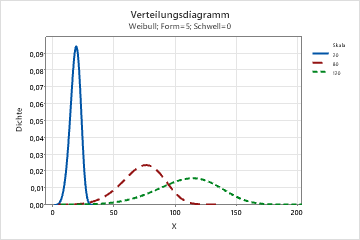
\includegraphics[width=0.5\textwidth]{weibull_shape.png}
    \fbox{\parbox{0.5\textwidth}{\centering [Weibull Shape Parameter Plot]}}
    \caption{Weibull Shape Parameter Effect}
    \label{fig:weibull_shape}
\end{figure}

\begin{figure}[h]
    \centering
    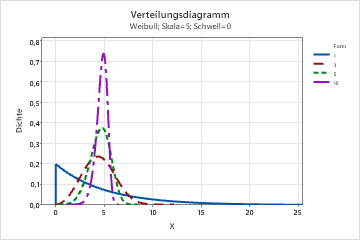
\includegraphics[width=0.5\textwidth]{weibull_scale.png}
    \caption{Weibull Scale Parameter Effect}
    \label{fig:weibull_scale}
\end{figure}

\begin{figure}[h]
    \centering
    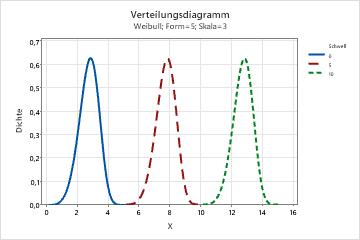
\includegraphics[width=0.5\textwidth]{weibull_location.png}
    \caption{Weibull Location Parameter Effect}
    \label{fig:weibull_location}
\end{figure}

\section{Distribution Characteristics}

\begin{itemize}
    \item \textbf{Skewness}: Third standardized moment, measures asymmetry
    \begin{equation}
        \text{Skewness} = \frac{\mathbb{E}[(X-\mu)^3]}{\sigma^3}
    \end{equation}
    \begin{itemize}
        \item $= 0$: Symmetric distribution
        \item $> 0$: Right-skewed (tail extends right)
        \item $< 0$: Left-skewed (tail extends left)
    \end{itemize}

    \item \textbf{Excess Kurtosis}: Fourth standardized moment minus 3, measures tail heaviness
    \begin{equation}
        \text{Excess Kurtosis} = \frac{\mathbb{E}[(X-\mu)^4]}{\sigma^4} - 3
    \end{equation}
    \begin{itemize}
        \item $= 0$: Normal distribution tails
        \item $> 0$: Heavy tails (leptokurtic)
        \item $< 0$: Light tails (platykurtic)
    \end{itemize}
\end{itemize}

\section{Tolerance \& Coverage Metrics}

\begin{itemize}
    \item \textbf{\% $|$Distance$|$ > Threshold}: Fraction of points exceeding a specified tolerance (e.g., 1 cm)
    \item \textbf{\% Within $\pm2\sigma$}: Fraction within two standard deviations
    \item \textbf{Max $|$Distance$|$}: Maximum absolute deviation
    \item \textbf{Within Tolerance}: Fraction of values within user-defined tolerance bounds
\end{itemize}

\section{Agreement \& Comparison Metrics}

\subsection{Bland-Altman Analysis}
Used to assess agreement between two measurement methods or point clouds.

\begin{figure}[h]
    \centering
    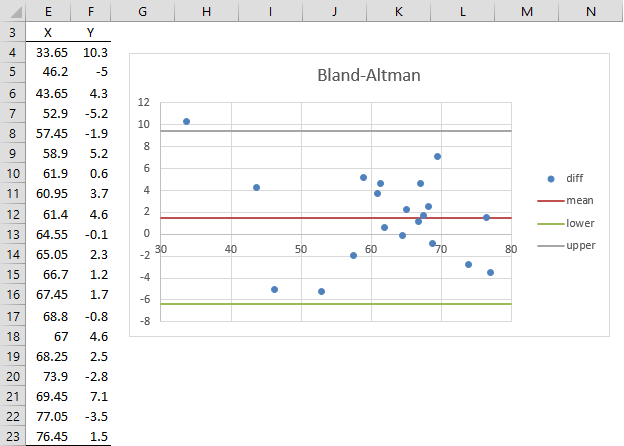
\includegraphics[width=0.7\textwidth]{bland_altman_example.png}
    \caption{Bland-Altman Plot Example}
    \label{fig:bland_altman}
\end{figure}

\begin{itemize}
    \item \textbf{x-axis}: Mean of both methods per data point
    \item \textbf{y-axis}: Difference between methods (typically Method A $-$ Method B)
    \item \textbf{Red line (Bias)}: Mean difference across all points
    \item \textbf{Green lines (Limits of Agreement)}: Bias $\pm$ 1.96 $\times$ SD
\end{itemize}

\textbf{Key Components:}
\begin{itemize}
    \item \textbf{Bias (Mean Difference)}: Systematic offset between methods
    \begin{equation}
        \text{Bias} = \bar{d} = \frac{1}{n}\sum_{i=1}^{n} d_i
    \end{equation}

    \item \textbf{Limits of Agreement (LoA)}: Expected range for 95\% of differences
    \begin{equation}
        \text{LoA} = \text{Bias} \pm 1.96 \times \sigma_d
    \end{equation}
    where $\sigma_d$ is the standard deviation of differences
\end{itemize}

\textbf{Interpretation:}
\begin{itemize}
    \item Bias $\approx$ 0: Methods agree on average
    \item Bias $\neq$ 0: One method consistently yields higher/lower results
    \item Narrow LoA: High agreement (low variance)
    \item Wide LoA: High uncertainty, poor reproducibility
    \item Random scatter: Differences independent of measurement magnitude (good)
    \item Patterns/trends: Systematic errors or heteroscedasticity (problematic)
\end{itemize}

\textbf{References:}
\begin{itemize}
    \item \url{https://en.wikipedia.org/wiki/Bland-Altman_plot}
    \item \url{https://pmc.ncbi.nlm.nih.gov/articles/PMC4470095/}
    \item \url{https://datatab.net/tutorial/bland-altman-plot}
\end{itemize}

\subsection{Passing-Bablok Regression}
Non-parametric method for comparing measurement methods, robust to outliers.

\textbf{Method:}
\begin{enumerate}
    \item Calculate slopes for all point pairs
    \item Take median slope ($\beta_1$) and median intercept ($\beta_0$)
    \item Compute confidence intervals
\end{enumerate}

\textbf{Interpretation:}
\begin{itemize}
    \item $1 \in$ CI(slope) AND $0 \in$ CI(intercept): Methods are comparable
    \item $1 \notin$ CI(slope): Proportional difference exists
    \item $0 \notin$ CI(intercept): Systematic difference exists
\end{itemize}

\section{Single-Cloud Statistics}

\subsection{Input Parameters}
\begin{itemize}
    \item \textbf{Radius [m]}: Search radius for local neighborhood analysis
    \item \textbf{k-NN}: Number of nearest neighbors for distance calculations
    \item \textbf{Sampled Points}: Number of randomly sampled points for computationally intensive metrics
    \item \textbf{Area Source}: Method for XY area estimation
    \begin{itemize}
        \item \texttt{convex\_hull}: Convex hull of 2D footprint (more realistic)
        \item \texttt{bbox}: Axis-aligned bounding box (overestimate)
    \end{itemize}
\end{itemize}

\subsection{Global Height Statistics (Z-dimension)}
\begin{itemize}
    \item \textbf{Z Min/Max [m]}: Elevation extrema
    \begin{equation}
        z_{\min} = \min(z), \quad z_{\max} = \max(z)
    \end{equation}

    \item \textbf{Z Mean/Median [m]}: Central tendency of elevation
    \begin{equation}
        \bar{z} = \frac{1}{N}\sum_{i=1}^{N} z_i
    \end{equation}
    Large mean-median difference indicates skewed distribution

    \item \textbf{Z Standard Deviation [m]}: Elevation variability
    \begin{equation}
        \sigma_z = \sqrt{\frac{1}{N-1}\sum_{i=1}^{N} (z_i - \bar{z})^2}
    \end{equation}

    \item \textbf{Z Quantiles [m]}: Robust elevation range descriptors
    \begin{itemize}
        \item Q05/Q95: Range excluding extreme 10\%
        \item Q25/Q75: Interquartile range (IQR)
    \end{itemize}
\end{itemize}

\subsection{Density Metrics}
\begin{itemize}
    \item \textbf{Global Density [pts/m$^2$]}: Overall point density
    \begin{equation}
        \rho_{\text{global}} = \frac{N}{A_{XY}}
    \end{equation}
    where $N$ = point count, $A_{XY}$ = footprint area

    \item \textbf{Local Density [pts/m$^3$]}: Neighborhood-based density
    \begin{equation}
        \rho_{\text{local}}(p) = \frac{|\mathcal{N}_r(p)|}{V_{\text{sphere}}}
    \end{equation}
    where $|\mathcal{N}_r(p)|$ = neighbor count, $V_{\text{sphere}} = \frac{4}{3}\pi r^3$
\end{itemize}

\subsection{k-Nearest Neighbor Statistics}
\begin{itemize}
    \item \textbf{Mean Distance to 1st-kth NN [m]}: Average distance to k nearest neighbors
    \begin{equation}
        \bar{d}_{1:k} = \frac{1}{M}\sum_{p \in S} \left(\frac{1}{k}\sum_{j=1}^{k} d_j(p)\right)
    \end{equation}

    \item \textbf{Mean Distance to kth NN [m]}: Scale indicator
    \begin{equation}
        \bar{d}_k = \frac{1}{M}\sum_{p \in S} d_k(p)
    \end{equation}
    Smaller values indicate denser sampling
\end{itemize}

\subsection{Surface Roughness}
\begin{itemize}
    \item \textbf{Roughness [m]}: Standard deviation of points from local best-fit plane
    \item Computed via PCA of local neighborhoods
\end{itemize}

\subsection{PCA Shape Descriptors}

Based on eigenvalue analysis of local point neighborhoods with eigenvalues $\lambda_1 \geq \lambda_2 \geq \lambda_3 \geq 0$:

\begin{itemize}
    \item \textbf{Linearity}: Degree of linear structure
    \begin{equation}
        L = \frac{\lambda_1 - \lambda_2}{\lambda_1}
    \end{equation}

    \item \textbf{Planarity}: Degree of planar structure
    \begin{equation}
        P = \frac{\lambda_2 - \lambda_3}{\lambda_1}
    \end{equation}

    \item \textbf{Sphericity}: Degree of isotropic distribution
    \begin{equation}
        S = \frac{\lambda_3}{\lambda_1}
    \end{equation}

    \item \textbf{Anisotropy}: Overall directional bias
    \begin{equation}
        A = \frac{\lambda_1 - \lambda_3}{\lambda_1}
    \end{equation}

    \item \textbf{Omnivariance [m$^2$]}: Geometric mean of eigenvalues
    \begin{equation}
        O = (\lambda_1 \lambda_2 \lambda_3)^{1/3}
    \end{equation}

    \item \textbf{Eigenentropy}: Disorder measure
    \begin{equation}
        H = -\sum_{i=1}^{3} p_i \log(p_i), \quad p_i = \frac{\lambda_i}{\sum_j \lambda_j}
    \end{equation}

    \item \textbf{Curvature}: Surface curvature indicator
    \begin{equation}
        \kappa = \frac{\lambda_3}{\lambda_1 + \lambda_2 + \lambda_3}
    \end{equation}
\end{itemize}

\subsection{Orientation Metrics}
\begin{itemize}
    \item \textbf{Verticality [degrees]}: Angle between local normal and vertical (Z-axis)
    \begin{equation}
        \theta = \arccos(|n_z|) \times \frac{180^\circ}{\pi}
    \end{equation}
    \item \textbf{Normal Standard Deviation [degrees]}: Consistency of normal orientations
\end{itemize}

\end{document}